% Fusing two paths: gamma_1 from gamma_1(0) to gamma_1(1)=gamma_2(0), then gamma_2.
% Source: book/tex/topology/fundamental-group.tex (§ Fusing paths together).
\documentclass[border=2mm]{standalone}
\usepackage{tikz}
\usetikzlibrary{arrows.meta}
\begin{document}
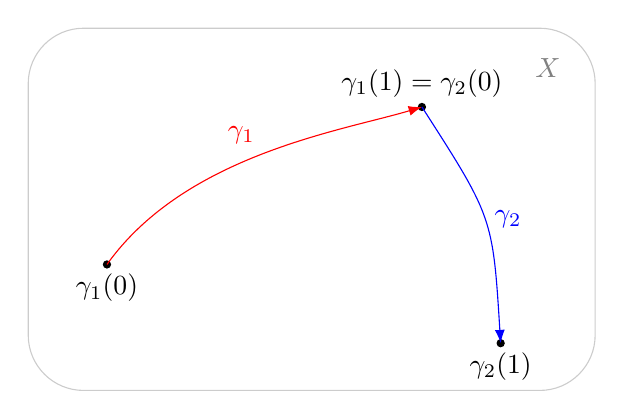
\begin{tikzpicture}[scale=1]
  \draw[rounded corners=20pt, gray!40] (-4,-2.6) rectangle (3.2,2);
  \node[gray] at (2.6,1.5) {$X$};
  \coordinate (A) at (-3,-1);
  \coordinate (B) at (1,1);
  \coordinate (C) at (2,-2);
  \fill (A) circle (1.5pt) node[below] {$\gamma_1(0)$};
  \fill (B) circle (1.5pt) node[above] {$\gamma_1(1)=\gamma_2(0)$};
  \fill (C) circle (1.5pt) node[below] {$\gamma_2(1)$};
  \draw[red,-{Latex}] (A) .. controls (-2,0.4) and (0,0.7) .. (B)
    node[midway,above left,red] {$\gamma_1$};
  \draw[blue,-{Latex}] (B) .. controls (1.9,-0.4) .. (C)
    node[midway,right,blue] {$\gamma_2$};
\end{tikzpicture}
\end{document}
